\documentclass{article}
\usepackage[dutch]{babel}

\usepackage[utf8]{inputenc}
\usepackage{geometry}
\usepackage[colorlinks=true, allcolors=blue]{hyperref}
\geometry{
  a4paper,
  total={170mm,257mm},
  left=20mm,
  top=20mm,
}
\usepackage{graphicx}
\usepackage{float}
\usepackage{titling}



\usepackage{amsfonts}
\title{Bucket Sort}


% Use the package to disaply c++ code 
\usepackage{listings}
\usepackage{xcolor}


\lstloadlanguages{[Visual]C++, [ISO]C++}

\definecolor{codegreen}{rgb}{0,0.7,0}
\definecolor{codegray}{rgb}{0.5,0.5,0.5}
\definecolor{codepurple}{rgb}{0.58,0,0.82}
\definecolor{backcolour}{rgb}{0.95,0.95,0.92}

\lstdefinestyle{mystyle}{
  language={[Visual]C++},
  backgroundcolor=\color{white},   
  commentstyle=\color{codegreen},
  keywordstyle=\color{blue},
  numberstyle=\tiny\color{codegray},
  stringstyle=\color{brown},
  basicstyle=\ttfamily\footnotesize,
  breakatwhitespace=false,         
  breaklines=true,                 
  captionpos=b,                    
  keepspaces=true,                 
  numbers=left,                    
  numbersep=5pt,                  
  showspaces=false,                
  showstringspaces=false,
  showtabs=true,                  
  tabsize=2,
  morekeywords=[2]{pow, emplace_back, static_cast, size, vector, push_back, insert, begin, end},
  keywordstyle=[2]\color{red},
}

\lstset{style=mystyle}

\author{Stan Merlijn}
\date{februari 2025}
 
\usepackage{fancyhdr}
\fancypagestyle{plain}{%  the preset of fancyhdr 
    \fancyhf{} % clear all header and footer fields
    % \fancyfoot[R]{\includegraphics[width=2cm]{KULEUVEN_GENT_RGB_LOGO.png}}
    \fancyfoot[L]{\thedate}
    \fancyfoot[C]{\thepage}
    \fancyhead[L]{Bucket Sort summary}
    \fancyhead[R]{}
}

\makeatletter
\def\@maketitle{%
  \newpage
  \null
  \vskip 1em%
  \begin{center}%
  \let \footnote \thanks
    {\LARGE \@title \par}%
    \vskip 1em%
    %{\large \@date}%
  \end{center}%
  \par
  \vskip 1em}
\makeatother

\usepackage{lipsum}
% \usepackage{cmbright}

\begin{document}

\maketitle

\noindent\begin{tabular}{@{}ll}
    Student & \theauthor\\
    Email & stan.merlijn@student.hu.nl \\
    Studentennummer & 1863967 \\
    link github & \url{https://github.com/StanMerlijn/HPP-bucket-Sort.git} \\
     % Promotor &  dr. Gilles Callebaut\\
     % Co-promotors & ing. Jarne Van Mulders, ing. Guus Leenders
\end{tabular}

\section{Inleiding}
In deze opdracht wordt het bucket sort-algoritme geïmplementeerd. Voor negatieve positieve getallen en comma getallen.
Het doel van deze opdracht is om het bucket sort-algoritme te implementeren en te testen met verschilende groottes van arrays.
\section{aanpak}
\subsection{1. Distribution pass}
De eerste stap van het bucket sort-algoritme is de distribution pass. In deze stap wordt de input array verdeeld in verschilende buckets.
Zowel voor de gehelle getallen als voor de kommagetallen is er een aparte functie geschreven. 

De functies zijn hieronder te zien. het enige verschil tussen de twee functies is dat de \texttt{float} functie de input array eerst cast naar een int en daarna de digit berekent. 
De functie om de digit te bereken: 
\begin{lstlisting}[caption={digit berekenen}, label={lst:digit}]
  int digit = (num / int(std::pow(10, i))) % 10;
\end{lstlisting}
Waar:
\begin{itemize}
  \item[-] num: het getal dat in het bucket moet worden geplaatst
  \item[-] i: de index van de digit waar het getal op moet worden gesorteerd 0 is de laatste digit.
\end{itemize}
Deze functie haalt de digit van het getal op de i-de plaats. Dit geld voor gehelle getallen. 
Voor kommagetallen wordt het getal eerst gecast naar een \texttt{int} en daarna de digit berekent. Dit verliest wel de decimalen van het getal. 
Daarom worden de kommagetallen eerst geschaald met een factor. Met dit cijfer kan het getal in de overeenkomstige bucket geplaatst worden.

\begin{lstlisting}[caption={Distribution pass}, label={lst:distribution}]
  void distributePassInt(std::vector<int>& input, std::vector<std::vector<int>>& buckets, int i)
  {
      for (int j = 0; j < input.size(); j++) {
          int num = input[j];
          int digit = (num / int(std::pow(10, i))) % 10;
          buckets[digit].emplace_back(num);
      }
  }

  void distributePassFloat(std::vector<float>& input, std::vector<std::vector<float>>& buckets, int i)
  {
      for (int j = 0; j < input.size(); j++) {
          int num = static_cast<int>(input[j]);
          int digit = int(num / int(std::pow(10, i))) % 10;
          buckets[digit].emplace_back(num);
      }
  }
\end{lstlisting}
\subsection{2. gathering pass}
In de gathering pass worden de buckets weer samengevoegd tot één array. Deze functie is voor zowel gehele getallen als kommagetallen identiek, 
waardoor er gebruik wordt gemaakt van templates. Hiermee wordt van een 2D-array een 1D-array gecreëerd.

\newpage
\begin{lstlisting}[caption={Gathering pass}, label={lst:gathering}]
  template<typename T>
  std::vector<T> gatheringPass(const std::vector<std::vector<T>>& input)
  {       
      std::vector<T> output;
      for (int i = 0; i < input.size(); i++) {
          for (int j = 0; j < input[i].size(); j++){
              output.emplace_back(input[i][j]);
          }
      }
    return output;
  }
\end{lstlisting}
\subsection{3. Negatieve getallen}
Om negatieve getallen te sorteren, worden de negatieve en positieve getallen eerst gescheiden.  
De negatieve getallen worden omgezet naar positieve waarden en vervolgens gesorteerd met behulp van het Bucket Sort-Algoritme; 
hetzelfde geldt voor de positieve getallen.
\begin{lstlisting}[caption={Negatieve getallen}, label={lst:negatives}]
  // NOTE: dit is voor integers
  std::vector<T> negatives, nonNegatives;
  for (auto num : input) {
      if (num < 0) {
          // Store the absolute value for sorting the negatives
          negatives.push_back(-num);
      } else {
          nonNegatives.push_back(num);
      }
  }
  // NOTE: dit is voor floats ze worden geschaald met een factor
  std::vector<T> negatives, nonNegatives;
  for (auto num : input) {
      if (num < 0) {
          negatives.push_back(-num * scaleFactor);
      } else {
          nonNegatives.push_back(num * scaleFactor);
      }
  }
\end{lstlisting}

De originele negatieve vector wordt vervolgens omgedraaid, 
omdat de negatieve getallen (na omzetting naar positieve waarden) in omgekeerde volgorde zijn gesorteerd. 
Hierdoor staat het oorspronkelijk grootste (in absolute waarde) getal als eerste.  
Bijvoorbeeld: de getallen \(-1\), \(-2\) en \(-3\) worden na omzetting en sortering als \(3\), \(2\), \(1\) gerangschikt. 
Daarna worden beide verzamelingen samengevoegd. Het samen voegen gebeurd zowel voor gehele getallen als kommagetallen op dezelfde manier.
\begin{lstlisting}[caption={getallen samenvoegen}, label={lst:negatives}]
  // Concatenate the negative and non-negative numbers
  negatives.insert(negatives.end(), nonNegatives.begin(), nonNegatives.end());

  // Divide each float by scaleFactor
  for (int i = 0; i < negatives.size(); i++) {
      negatives[i] = negatives[i] / scaleFactor;
  }
  return negatives;  
\end{lstlisting}



\subsection{4. Comma getallen}
Zoals eerder vermeld worden de kommagetallen van de input vector geschaald met een \hyperref[lst:negatives]{factor}. 
Deze factor is op het moment 1000.0f dit betekent dat de kommagetallen worden geschaald met 3 decimalen. 
Dit kan er voor zorgen dat de kommagetallen precisie verliezen. Dit is een trade-off tussen snelheid en precisie.

\begin{lstlisting}[caption={Terug schalen}, label={lst:factor}]
  for (int i = 0; i < negatives.size(); i++) {
            negatives[i] = -negatives[i];
        }
\end{lstlisting}

\newpage
\section{complexiteitsanalyse}
Om het Bucket Sort-Algoritme te testen, is het algoritme met arrays van verschillende groottes uitgevoerd; voor elke grootte is het algoritme 100 keer gerund.  
De resultaten zijn in de onderstaande grafiek weergegeven. Deze grafiek toont aan dat het Bucket Sort-Algoritme een tijdcomplexiteit van \(O(n)\) heeft.

Hieronder zie je de resultaten van de Bucket Sort-benchmark (CLI-output). 
‘Est. Run Time’ geeft de geschatte totale uitvoeringstijd weer, 
‘Mean’ is de gemiddelde tijd die het algoritme nodig heeft over de 100 uitvoeringen en ‘Std Dev’ geeft de standaardafwijking van de meetwaarden aan.

\begin{table}[H]
  \caption{Bucket Sort Benchmark Results: Large \texttt{ints} (detailed)\label{tab:ints-detailed}}
  \begin{tabular*}{\columnwidth}{@{\extracolsep\fill}lccccc}
    \hline
    Benchmark  & Iter. & Est. Run Time & Mean          & Std Dev       \\
    \hline
    Bucket Sort 10     & 2 & 4.4852 ms  & 22.4083 us  & 808.702 ns  \\
    Bucket Sort 100    & 1 & 7.7749 ms  & 78.0013 us  & 1.56197 us  \\
    Bucket Sort 1000   & 1 & 45.5004 ms & 455.9 us    & 2.43898 us  \\
    Bucket Sort 10000  & 1 & 589.814 ms & 5.89859 ms  & 28.6057 us  \\
    Bucket Sort 100000 & 1 & 5.55511 s  & 55.6646 ms  & 253.145 us  \\
    \hline
  \end{tabular*}
\end{table}

\begin{table}[H]
  \caption{Bucket Sort Benchmark Results: Large \texttt{floats} (detailed)\label{tab:floats-detailed}}
  \begin{tabular*}{\columnwidth}{@{\extracolsep\fill}lccccc}
    \hline
    Benchmark  & Iter. & Est. Run Time & Mean          & Std Dev       \\
    \hline
    Bucket Sort 10     & 1 & 3.3439  ms  & 33.6925 us  & 1.27137  us  \\
    Bucket Sort 100    & 1 & 12.4503 ms & 126.133  us  & 2.4091  us   \\
    Bucket Sort 1000   & 1 & 82.2361 ms & 811.04   us  & 3.01316 us  \\
    Bucket Sort 10000  & 1 & 819.995 ms & 8.16308  ms  & 40.902  us   \\
    Bucket Sort 100000 & 1 & 7.74322 s  & 77.2987  ms  & 274.485 us  \\
    \hline
  \end{tabular*}
\end{table}

\vspace{1em}

Uit deze resultaten is de est run time er uit gehaald en geplot tegen de grootte van de array:
\begin{figure}[H]
    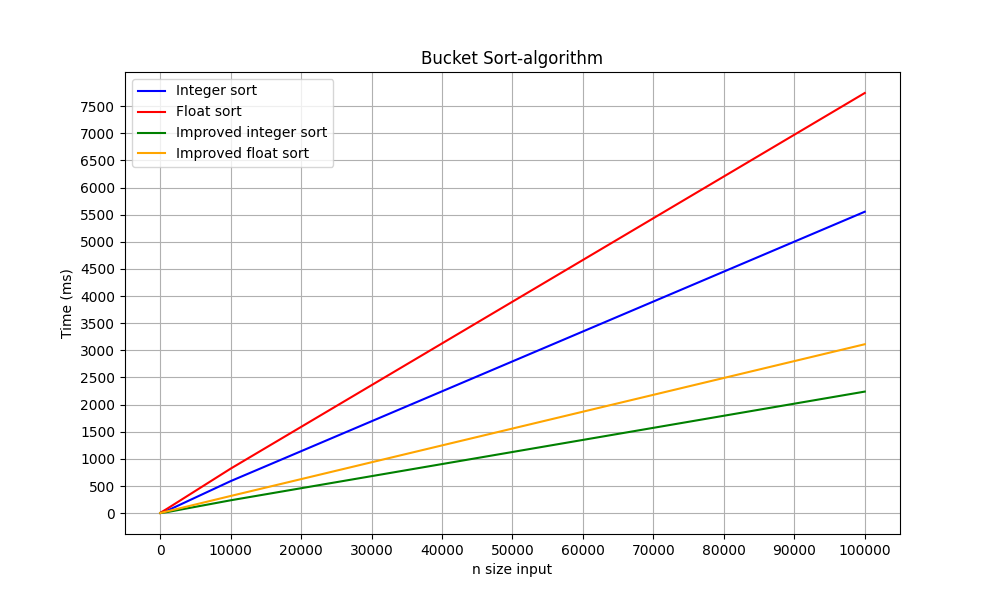
\includegraphics[width=1\textwidth]{images/bucket_sort.png}
    \caption{Complexity of the bucket sort-algoritme}
    \label{fig:complexity}
\end{figure}

\section{Performance}
\begin{itemize}
\item[-] \textbf{Distributiepass:} \\
Elke distributiepass scant het gehele inputarray en plaatst elk element in één van de 10 buckets. Dit levert een tijdcomplexiteit van O(n) per pass op.

\item[-] \textbf{Gathering pass:} \\
In de gathering pass worden alle buckets samengevoegd in één vector. Dit kost ook O(n) per pass.

\item[-] \textbf{Aantal passes:} \\
Het totale aantal passes wordt bepaald door het aantal cijfers (digit count) van het maximale element. In het slechtste geval (bijvoorbeeld voor grote aantallen) is dit $\log_{10}(\mathrm{max})$ wat vrij beperkt blijft, zodat de overhead laag is.

\item[-] \textbf{Extra bewerkingen:} \\
Voor negatieve getallen wordt er een extra stap uitgevoerd voor het omkeren en weer aanvullen van de negatieve subvector.
Voor kommagetallen wordt er een schaaloperatie uitgevoerd vóór en na het sorteren. Deze stappen zijn lineair en hebben een kleine constante extra kost.
\end{itemize}
\end{document}